\chapter{Opis projektnog zadatka}
		Cilj ovog projekta je razviti programsku podršku za stvaranje web aplikacije "Ozdravi" koja će služiti za povezivanje roditelja s medicinskim stručnjacima poput pedijatara i liječnika. Aplikacija ima za cilj olakšati komunikaciju, štedjeti vrijeme i ubrzati proces pregleda oboljele djece.
		
		Roditeljima će aplikacija omogućiti jednostavan pristup informacijama o zdravlju njihovog djeteta, uključujući povijest bolesti, preporuke liječnika te prijavu samih pregleda djeteta online putem. Liječnicima i pedijatrima će aplikacija pružiti bolji uvid u medicinsku povijest djece omogućujući im brže donošenje odluka, pregledavanje, planiranje i organizaciju pristiglih zahtjeva za pregled djece te slanje povratnih informacija i dokumenata roditeljima bez potrebe fizičkog posjeta roditelja za preuzimanje istih. Za administratorski pristup aplikaciji, omogućit će se širok spektar ovlasti kako bi administrator imao potpunu kontrolu i pristup svim podacima. Samim time administrator može nadzirati, otkriti i ukloniti nastale probleme jednostavnim putem te tako održavati web aplikaciju i pružati njezinim korisnicima brzu i efikasnu korisničku podršku. Sve zajedno će doprinijeti efikasnijem i transparentnijem procesu brige o zdravlju djece te olakšati život svi sudionika u tom procesu.
		
		Ciljana publika ove aplikacije su zauzeti, zaposleni roditelji s više djece koji su često na bolovanju zbog nemogućnosti interakcije između svih instanci u zdravstvu. Time su prisiljeni izostati iz posla, a djecu iz škole ili vrtića što uzrokuje stres i gubitak dragocjenog vremena čekajući po raznim natrpanim čekaonicama. Također, aplikacija je namijenjena liječnicima i pedijatrima koji žele olakšati svoj posao i povećati produktivnost. Korištenjem aplikacije oni ubrzavaju pregled dobivenih nalaza pacijenata, planiranje samog pregleda te slanje povratnih informacija roditeljima.
		
		\textbf{Neregistriranom korisniku} je omogućeno prijavljivanje u sustav s postojećim računom unosom lozinke i email adrese ili kreiranjem novog računa. Za kreiranje novog računa potrebni su sljedeći podaci: 
				\begin{packed_item}
					\item ime
					\item prezime
					\item spol
					\item datum rođenja
					\item adresa
					\item email
					\item lozinka
				\end{packed_item}
		
			\textbf{Roditeljima} je omogućeno pregledavanje naslovne stranice s novim obavijestima i zakazanim terminima pregleda, pregledavanje vlastitog profila, profila djece i povijesti pregleda, prijava željenog termina pregleda te slanje privatnih nalaza pregleda direktno liječniku/pedijatru.
		
		\textbf{Liječnicima/pedijatrim} je omogućeno pregledavanje dolaznih zahtjeva za preglede, popisa pacijenata, kreiranje novih zapisa pregleda, izdavanje ispričnica i molbi za bolovanje te brisanje i uređivanje prijašnjih pregleda pacijenata.
		
			\textbf{Administratorima} je omogućeno uređivanje osobnih podataka korisnika, brisanje samih korisnika, mijenjanje njihovih uloga, te brisanje i uređivanje pregleda pacijenata.
		
		Najpoznatija postojeća slična rješenja su ChARM Health i MyChart. MyChart je aplikacija razvijena od strane tvrtke Epic Systems Corporation, američke privatne tvrtke za razvoj softvera u području zdravstva. Ona pruža sigurnu online platformu koja omogućuje pacijentima pristup osobnim zdravstvenim informacijama i komunikaciju s njihovim zdravstvenim ustanovama. Neke od značajnijih zajedničkih stavki aplikacija Ozdravi i MyChart čine:
		
		\begin{packed_enum}
			\item Pristup medicinskim zapisima pacijenta
			\begin{itemize}
				\item mogućnost čuvanja i pregledavanja medicinske povijesti pacijenata
			\end{itemize}
			\item Zakazivanje termina
				\begin{itemize}
				\item omogućuju dogovor i zakazivanje termina pregleda slanjem upita liječniku
			\end{itemize}
			\item Pregled zdravstvenih profila
			\begin{itemize}
				\item mogućnost pohrane i pregleda korisničkih profila roditelja i djece
			\end{itemize}
			\item Izravno slanje medicinskih dokumenata
			\begin{itemize}
				\item pacijenti imaju mogućnost izravnog slanja novih nalaza zdravstvenoj ustanovi
			\end{itemize}
		\end{packed_enum}
		
		Nadalje, MyChart sadrži dodatne implementirane stavke koje nisu dio Ozdravi aplikacije:
		\begin{packed_enum}
			\item Stanje računa i plaćanje
			\begin{itemize}
				\item pacijenti mogu pregledavati i plaćati svoje medicinske račune
			\end{itemize}
			\item Integracija telekomunikacijskih tehnologija
			\begin{itemize}
				\item MyChart je integriran s telezdravstvenim uslugama omogućavajući pacijentima virtualne konzultacije
			\end{itemize}
			\item Podsjetnik o uzimanju ljekova
			\begin{itemize}
				\item aplikacija implementira praćenje doza uzimanih ljekova i dnevne podsjetnike o uzimanju istih
			\end{itemize}
		\end{packed_enum}

		\begin{figure}[H]
			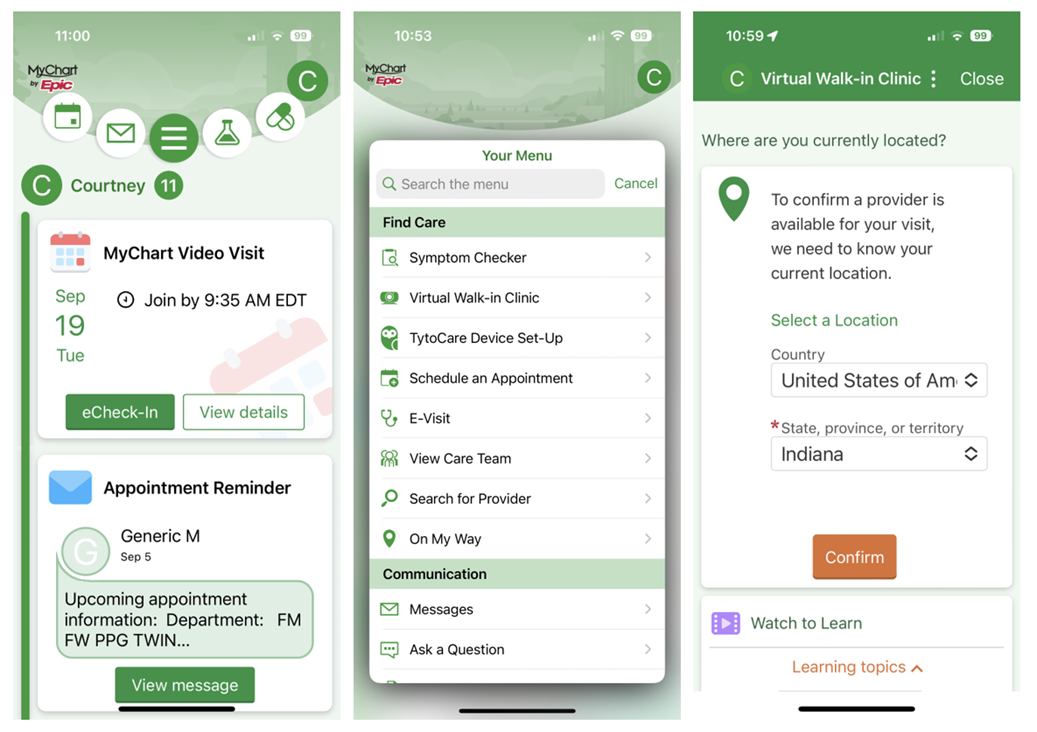
\includegraphics[scale=0.4]{slike/myChartMobileView.PNG}
			\centering
			\caption{MyChart mobilno sučelje}
			\label{fig:myChart}
		\end{figure}
		
		Projektni zadatak se nadalje može nadograditi dodavanjem:
		
		\begin{packed_item}
			\item geografskih mapa najbližih dostupnih zdravstvenih ustanova prilikom hitnih slučajeva
			\item forum portala za međusobnu komunikaciju svih korisnika aplikacije
			\item sustava za povratne informacije o iskustvima korisnika
			\item integracije s nosivim uređajima
			\item integracije s telezdravstvenim uslugama pojedinih zdravstvenih ustanova
			\item mogućnosti elektroničkih zahtjeva recepata
		\end{packed_item}